% Fig. 2 — Label efficiency (values from benchmarks)
\begin{figure}[t]
\centering
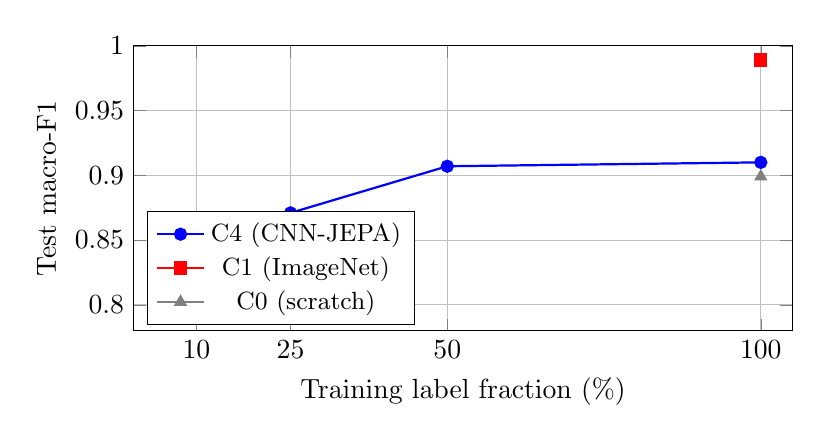
\begin{tikzpicture}
\begin{axis}[
  width=0.82\linewidth,
  height=5.2cm,
  xlabel={Training label fraction (\%)},
  ylabel={Test macro-F1},
  xmin=0, xmax=105,
  ymin=0.78, ymax=1.0,
  xtick={10,25,50,100},
  legend style={at={(0.02,0.02)}, anchor=south west, font=\small},
  grid=major,
]
\addplot[mark=*, thick, blue] coordinates {
  (10, 0.825) (25, 0.871) (50, 0.907) (100, 0.910)
};
\addlegendentry{C4 (CNN-JEPA)}
\addplot[mark=square*, thick, red] coordinates {
  (100, 0.989)
};
\addlegendentry{C1 (ImageNet)}
\addplot[mark=triangle*, thick, gray] coordinates {
  (100, 0.899)
};
\addlegendentry{C0 (scratch)}
\end{axis}
\end{tikzpicture}
\caption{Label-efficiency curve on the Simula fold. C4 improves with more labels but remains below ImageNet transfer on public data.}
\label{fig:labelcurve}
\end{figure}
